\documentclass[aspectratio=169]{beamer}
\usepackage{amssymb,amsmath}
\usepackage{graphicx}
\usepackage{url}
\usepackage{color}
\usepackage{pagenote}[continuous,page]
\usepackage{cancel}   % Math "cancelto"
\usepackage{relsize}	% For \smaller
\usepackage{url}			% For \url
\usepackage{epstopdf}	% Included EPS files automatically converted to PDF to include with pdflatex

%For MindMaps
\usepackage{tikz}%
\usetikzlibrary{mindmap,trees,arrows}%

%%% Color Definitions %%%%%%%%%%%%%%%%%%%%%%%%%%%%%%%%%%%%%%%%%%%%%%%%%%%%%%%%%
%\definecolor{bordercol}{RGB}{40,40,40}
%\definecolor{headercol1}{RGB}{186,215,230}
%\definecolor{headercol2}{RGB}{80,80,80}
%\definecolor{headerfontcol}{RGB}{0,0,0}
%\definecolor{boxcolor}{RGB}{186,215,230}

%%% Save space in lists. Use this after the opening of the list %%%%%%%%%%%%%%%%
%\newcommand{\compresslist}{
%	\setlength{\itemsep}{1pt}
%	\setlength{\parskip}{0pt}
%	\setlength{\parsep}{0pt}
%}

%\setbeameroption{show notes on top}

% You should run 'pdflatex' TWICE, because of TOC issues.

% Rename this file.  A common temptation for first-time slide makers
% is to name it something like ``my_talk.tex'' or
% ``john_doe_talk.tex'' or even ``discrete_math_seminar_talk.tex''.
% You really won't like any of these titles the second time you give a
% talk.  Try naming your tex file something more descriptive, like
% ``riemann_hypothesis_short_proof_talk.tex''.  Even better (in case
% you recycle 99% of a talk, but still want to change a little, and
% retain copies of each), how about
% ``riemann_hypothesis_short_proof_MIT-Colloquium.2000-01-01.tex''?

\mode<presentation>
{
  \usetheme{CambridgeUS}
  \usecolortheme{dolphin}
  \useoutertheme{default}
  \useinnertheme{default}
  \setbeamercovered{invisible} % or whatever (possibly just delete it)
}
\beamertemplatenavigationsymbolsempty

\usepackage[english]{babel}
%\usepackage[latin1]{inputenc}
\usepackage{subfigure}

\usepackage{times}
\usepackage[T1]{fontenc}
\usepackage{CJKutf8}

%% makes the ppagenote command for figure references at the end.
\makepagenote
\renewcommand{\notenumintext}[1]{}
\newcommand{\ppagenote}[1]{\pagenote[Page \insertframenumber]{#1}}

\title[Experiment Design (01CH740)]{Experiment Design for Computer Sciences (01CH740)}
\author[Claus Aranha]{Claus Aranha\\{\footnotesize caranha@cs.tsukuba.ac.jp}}
\institute[U. Tsukuba]{University of Tsukuba, Department of Computer Sciences}


\subtitle[Intro]{Topic 00 - Course Introduction}

\begin{document}
\begin{CJK}{UTF8}{ipxm}


\begin{frame}
  \maketitle

  \vfill

  \hfill Version 2021.1
\end{frame}

\section{Course Motivation}
\begin{frame}{What is this course about?}

  \begin{block}{From the syllabus}
  \emph{The collection and analysis of data through experiments is one of the cornerstones of the scientific method. In this course, we study the general philosophy and methods behind experimentalism: Why do we perform experiments, what is a good/rigorous experiment, how to plan and design a rigorous experiment, and how to perform statistical analysis on experimental data.}
  \end{block}
  \bigskip

  ... {\bf TL;DR?}
\end{frame}

\begin{frame}{What is this course about?}{TL;DR; (Too Long, Didn't Read)}

  The key idea of this course is to learn how to \structure{plan, execute, analyse and interpret} a scientific experiment.\bigskip

  Another way to think is: "Experiment Design" is how to apply the PDCA cycle for science.
  \begin{center}
    \includegraphics[width=.6\textwidth]{../img/irasutoya_pdca}\ppagenote{PDCA flowchart from \url{https://www.irasutoya.com}}
  \end{center}
\end{frame}

\begin{frame}{What is this course about?}{Why is a course on "Experiment Design" necessary?}
  There are some common errors that I see from students many times:
  \bigskip

  \begin{itemize}
    \item The experiment does control for noise factors;\\
      \structure{Is the result just a coincidence?}
    \item The experiment that compare two methods is not fair;\\
      \structure{Is the new method really better than the old one?}
    \item The experiment is not reproducible;\\
      \structure{How can this experiment help other people?}
    \item The conditions and assumptions of the experiment are not clear;\\
      \structure{The results and conclusions are questionable}
    \item etc...
  \end{itemize}
\end{frame}

\begin{frame}{What is this course about?}{The "Dark Curriculum"}

  The \structure{Dark Curriculum} are things that are necessary for your work as an academic, but that you usually can't learn in a lecture, and must discover by \alert{trial and error}. For example:\bigskip

  \begin{columns}
    \column{0.7\textwidth}
    \begin{itemize}
      \item How do I prepare an experiment?
      \item When do I publish a result?
      \item How do I review a paper?
      \item How do I teach a lecture?
      \item What are grants?
      \item ...
    \end{itemize}\bigskip

    The goal of this course is to shed light in one of these points:\\
    \emph{What is an experiment, and how do I prepare it?}.\bigskip

    \column{0.3\textwidth}
    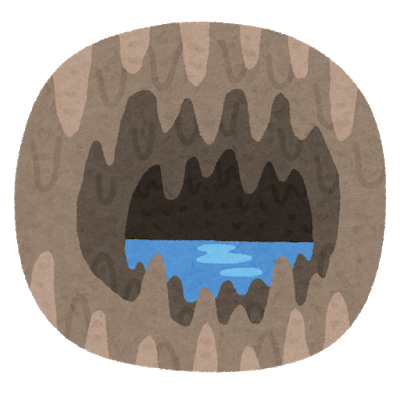
\includegraphics[width=1\textwidth]{../img/irasutoya_cave}\ppagenote{Cave illustration from \url{https://www.irasutoya.com}}
  \end{columns}
  \bigskip

\end{frame}

\section{Course Topics}
\begin{frame}{Course Topics}
  The main things that you will learn in this course are:\bigskip

  \begin{itemize}
    \item What is an experiment:
    \begin{itemize}
      \item What is the role of an experiment in Science?
      \item How do I design an experiment to answer a scientific question?
      \item What are the characteristics of a \structure{good} experiment?
      \item How do I analyse the results of an experiment?
    \end{itemize}\bigskip

    \item Statistical tools for analyzing experimental data:
    \begin{itemize}
      \item Basic statistics for data analysis and visualization;
      \item Statistical Inference ("Statistically Significant Results");
      \item Statistical testing for single, paired, and multiple sample testing;
      \item How to calculate the sample size and power of an experiment;
    \end{itemize}
  \end{itemize}
\end{frame}

\begin{frame}{Course Topics}{Limitations: This is only an introductory course!}

  \begin{columns}
    \column{0.8\textwidth}
    This course is an \structure{introduction} to design of experiment. My main objective is to teach you {\bf why} designing experiments is important, and what problems can happen when you don't do this. Not to teach all the statistical tests.
    %\column{0.1\textwidth}
    \column{0.2\textwidth}
      \includegraphics[width=1\textwidth]{../img/irasuto_sprout}
      \ppagenote{Sprout image from \url{https://www.irasutoya.com}}
  \end{columns}
  \vfill

  Each experiment, in each research, will require a different way of doing statistical analysis. Also, some advanced topics (bayesian statistical analysis) will not be covered here. I hope that after this course you will have a solid understanding of the concepts to read and learn the advanced tests required of your own research.
\end{frame}

\section{Practical Details}
\begin{frame}
  \frametitle{Practical Details about the course}
  \begin{itemize}
    \item Teaching Format;
    \item Course Materials;
    \item Course Schedule;
    \item Grading;
    \item Course Policy;
  \end{itemize}\vfill

  \alert{Note}: these details have small differences from the syllabus. The latest information is always on manaba.
\end{frame}

\subsection{Course Format}
\begin{frame}{Course Format (Fri, 15:15 to 18:00)}
  \begin{block}{Online (On demand) Format}
    Video lectures and lecture notes published on manaba by the official lecture time. Please read the video lecture in full, at the time of your preference.
    \bigskip

    During the official lecture time, I will hold "office hours" on TEAMS. A link will be on manaba (I hope! :-)).
  \end{block}

  \begin{alertblock}{Two Exceptions:}
    Last class (06/18) is an online presentation of the final report. If you have problems with live presentation (time zones, etc), lemme know.\bigskip

    Final exam (06/25) will be live (online or in person, depends on covid situation in June). Tell me if you have timezone problems.
  \end{alertblock}
\end{frame}

\begin{frame}{Course Format}{Student / Teacher communication}
  \begin{itemize}
    \item \structure{Office hours}: Friday, 15:15-18:00, TEAMs meeting.\bigskip

    \item \structure{manaba Forums}: This is the preferred way for asynchronous communication, since all students can see the question. Other students are highly encouraged to answer or add their opinions.\bigskip

    \item \structure{e-mail}: If you need to ask a private question.
  \end{itemize}\bigskip

  One goal of this course is to shed light on the "Dark Curriculum". Please feel free to ask any questions at all about life as a scientist / academic / etc.
\end{frame}

%Teaching Format;
%Course Materials;

\subsection{Course Materials}
\begin{frame}{Course Materials}
  Required materials are posted on the "manaba" system. If you want to follow the course, but not take credit, you can access the manaba materials using the self-registration number: \structure{4054723}.
  \bigskip

  If you cannot access manaba, the course is also available on the following github repository: (not official) \url{https://caranha.github.io/ExperimentDesignCS/}.
  \bigskip

  Report submission, and some recommended readings are only available on manaba.
\end{frame}

\begin{frame}{Course Materials}{Lecture Notes}
  The main materials for this course are these lecture notes.
  Make sure to read them and ask questions if anything is unclear!
  \bigskip

  \begin{columns}
    \column{0.8\textwidth}
    The lecture notes were produced based on the "Design and Analysis of Experiments" material produced by Felipe Campelo. You can reach the original lecture notes on: \url{https://github.com/fcampelo/Design-and-Analysis-of-Experiments}

    \column{0.2\textwidth}
    \hfill\includegraphics[width=1\textwidth]{../img/Felipe_Campelo}
  \end{columns}
  \bigskip

  All good ideas are thanks to Felipe (and other contributors) all errors are my own :-) (Please submit errors as github issues!)
\end{frame}

\begin{frame}{Course Materials}{Books and Links}
  \begin{columns}
    \column{0.2\textwidth}
    \includegraphics[width=1\textwidth]{../img/DesignAnalysis_book}
    \column{0.8\textwidth}
    Many topics in this course are explored in much more depth on "Design and Analysis of Experiments", by Douglas C. Montgomery.
    \ppagenote{"Design and Analysis of Experiments" book cover image from Amazon.}
  \end{columns}
  \vspace{1cm}

  In manaba there will be an expanded list of resources for
  extra study. Make sure to check it out!
\end{frame}



\subsection{Course Schedule}
\begin{frame}{Course Schedule}{Friday, 15:15--18:00, no "change days"}
\begin{itemize}
  \item 4/09 : Introduction, What is Experimentation (Today)
  \item 4/16 : Point and Interval Indicators
  \item 4/23 : Inference Testing I
  \item 4/30 : Inference Testing II
  \item \alert{5/07 : Golden Week, no Class}
  \item 5/14 : R Tutorial / Review and Discussion of Project I
  \item 5/21 : Inference Testing III
  \item 5/28 : Case Studies: Inference Testing in CS papers
  \item 6/04 : Sample Size and Experiment Power
  \item 6/11 : Final Review
  \item 6/18 : Project II presentation
  \item 6/25 : \alert{Final Exam}
\end{itemize}
\end{frame}

%## Report 1 -- Simple Experiment
%- 04/20 Experiment Topic Submission
%- 05/09 Experiment Report Submission

%## Report 2 -- Experiment Analysis
%- 05/23 Experiment 2 Topic Submission
%- 06/18 Experiment 2 Presentation
%- 07/02 Experiment 2 Report Submission

\subsection{Grading}
\begin{frame}{Grading}
  Two reports (R1, R2), and a final examination (E). Each graded from 0 to 100.
  The final Grade (FG) is:

  \begin{equation*}
    FG = 0.2*R1 + 0.4*R2 + 0.4*E
  \end{equation*}
  \bigskip

  The letter grade for this course follows the Tsukuba standard ($< 60: D; < 70: C, < 80: B, < 90: A$)
\end{frame}

\begin{frame}{Grading}{Final Examination}
  \begin{itemize}
    \item Covers the topics of the entire course.
    \item Must be answered in English.
    \item You may prepare {\bf one A4 page of handwritten notes (both sides)}, and use it on the test.
    \begin{itemize}
      \item The notes have no fixed format, and can be in any language.
      \item The notes must include your name and student ID, and must be turned in with the exam. The notes will not be graded.
    \end{itemize}
    \item No other consultation is allowed in the exam.
    \item The exact format of the exam (online or in person), will be defined in June.
  \end{itemize}
\end{frame}

\begin{frame}{Grading}{Reports}
  Two "mini-papers". The student must plan, perform, and analyze an experiment of their own choice:\bigskip

  \begin{itemize}
    \item Choose a scientific question to answer
    \item Design an Experiment to gather data to answer that question
    \item Execute the experiment, following the design
    \item Analyze the data, following the design
    \item Make a conclusion, based on the analysis of the data
  \end{itemize}
\end{frame}

\begin{frame}{Grading}{Reports -- More Details}
  \begin{itemize}
    \item \structure{Report 1}: Choose a good experiment for a scientific question, and presenting the data (lectures 1 and 2). \bigskip
    \item \structure{Report 2}: Choose a proper hypothesis pre-data collection, and perform the appropriate inferential statistical test (lectures 1-7).
    \begin{itemize}
      \item Students must present their reports on lecture 10.
    \end{itemize}\bigskip
    \item \structure{Topic}: The experiment can be on any topic, but using the same topic as your research theme is recommended.
    \begin{itemize}
      \item If your research includes private data, consult with your advisor first.
    \end{itemize}\bigskip

    \item \structure{Important}: Your experiment will {\bf not} be judged based on the "success" of the experiment. Report your results honestly.
  \end{itemize}
\end{frame}

\begin{frame}{Grading}{Reports -- Final Details}
  \begin{itemize}
    \item Report must be in English.\bigskip
    \item Report text must be in pdf format.\bigskip
    \item In addition to the PDF, you must also submit all the information necessary to reproduce your experimental results.
    \begin{itemize}
      \item This depends on the experiment, but tipically include data files obtained from the experiment, and scripts used to process this data, generate figures and statistical tests.
      \item Data from the reports will be used only to evaluate the report, and deleted at the end of the course.
    \end{itemize}\bigskip
    \item Deadline for the reports will be posted on manaba.
  \end{itemize}
\end{frame}

\section{Others}
\begin{frame}{Other Topics:}{1 -- Computer Science English Program (CSE)}
  The CSE supports a master degree fully in English. If you plan to take most of your classes in Enslish, do not forget to enroll in the CSE:
  \bigskip

  Send an e-mail to \structure{s-g30@cs.tsukuba.ac.jp} with this info:
  \begin{itemize}
    \item Your name (ASCII and Kanji)
    \item Student ID
  \end{itemize}

  For more information, see the orientation material at the "New Student Orientation" course on manaba.
\end{frame}

\begin{frame}{Other Topics:}{2 -- Self Introduction}
  \begin{columns}
    \column{0.4\textwidth}
    \includegraphics[height=.8\textheight]{../img/pinhole}
    \column{0.6\textwidth}
    {\small
    \begin{itemize}
      \item \structure{Name:} Claus Aranha;
      \item \structure{Country:} Brazil;
      \item \structure{Research Topics:}
      \begin{itemize}
        \item Evolutionary Algorithms;
        \item Artificial Life;
      \end{itemize}
      \item \structure{Hobbies:}
      \begin{itemize}
        \item Game Programming;
        \item Geocaching;
      \end{itemize}
        \medskip

      \item \structure{webpage:}\\
      {\smaller \url{http://conclave.cs.tsukuba.ac.jp}}
      \medskip

      Ask me anything you want!
    \end{itemize}
    }
  \end{columns}
\end{frame}

\section{Backmatter}
\begin{frame}{About these Slides}
  These slides were made by Claus Aranha, 2022. You are welcome to copy, re-use and modify this material.
  \bigskip

  These slides are a modification of "Design and Analysis of Experiments (2018)" by Felipe Campelo, used with permission.
  \bigskip

  Individual images in some slides might have been made by other
  authors. Please see the following references for those cases.
\end{frame}

\begin{frame}[allowframebreaks]{Image Credits}
  \printnotes
\end{frame}

\end{CJK}
\end{document}
